\documentclass{scrbook}
\usepackage{siunitx}
\usepackage[version=4]{mhchem}
\usepackage{indentfirst}
\usepackage{tikz}
\usepackage{amsmath}
\usepackage{pgfplots}
\usepackage[backend=bibtex]{biblatex}
\usepackage{wrapfig}
\usetikzlibrary{positioning}
\addbibresource{Chemistry.bib}
\title{Physics Notes}
\subtitle{A level Chemistry}
\date{Last Updated \today{}}
\author{Dhruva Lokegaonkar}
\begin{document}
\maketitle
\tableofcontents

\chapter{Lattice Energy}

\section{What is Lattice Energy}

	The energy gicen out when ions of opposite charges come together to form a crystalline lattice. This is called the lattice energy, $\Delta H_{latt}^\ominus$.

	\[ \ce{Na+(g) + Cl-(g) ->  NaCl(s) \qquad \Delta H^\ominus_{latt} = \SI{-787}{ \kilo\joule\per\mole } }\]

	\begin{quote}
		Lattice energy is the enthalpy change when \SI{1}{\mole} of an ionic compound is formed from its gaseous ions under standard conditions.
	\end{quote}

	Lattice Energy is always negative. The value of lattice energy depends on the size of the ion and the ionic charge. As the ion size increases, or as ionic charge increases, lattice energy becomes more exothermic.

\section{Other Enthalpies}

\subsection{Enthalpy Change of Atomisation}

	\begin{quote}
		The standard enthalpy change of atomisation, $\Delta H_{at}^\ominus$, is the enthalpy change when \SI{1}{\mole} of gaseoues atoms is formed from it's elements under standard conditions.
	\end{quote}

	\[ \ce{ Li(s) -> Li(g) \qquad \Delta H^\ominus_{at} = \SI{161}{\kilo\joule\per\mole} } \]

	The Values of $\Delta H^\ominus_{at}$ are always positive.

\subsection{Electron Affinity}

	The energy change orrucing when a gaseous non metal atom accepts one electron is called the electron affinity. The symbol is $\Delta H^\ominus_{ea}$

	\begin{quote}
		The first electron affinity, $\Delta H^\ominus_{ea1}$, is the enthalpy when \SI{1}{\mole} of electrons is added to \SI{1}{\mole} of gaseous atoms to form \SI{1}{\mole} of gaseous atoms 1- ions under standard conditions.
	\end{quote}

	\[ \ce{ Cl(g) + e- -> Cl-(g) \qquad \Delta H^\ominus_{ea1} = \SI{-348}{\kilo\joule\per\mole} } \]

	$\Delta H^\ominus_{ea1}$ is usually negative.

	\begin{quote}
		The second electron affinity, $\Delta H^\ominus_{ea2}$, is the enthalpy when \SI{1}{\mole} of electrons is added to \SI{1}{\mole} of gaseous 1- ions to form \SI{1}{\mole} of gaseous atoms 2- ions under standard conditions.
	\end{quote}

	\[ \ce{ O-(g) + e- -> O^2-(g) \qquad \Delta H^\ominus_{ea2} = \SI{798}{\kilo\joule\per\mole} } \]

	$\Delta H^\ominus_{ea2}$ and $\Delta H^\ominus_{ea3}$ are always positive

\section{Born-Haber Cycle}

	\begin{wrapfigure}{R}{0.3\linewidth}
	\centering
	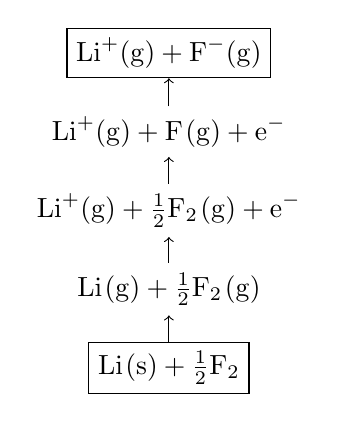
\begin{tikzpicture}[node distance=10mm]
		\node (a) [rectangle, draw] {$\ce{Li(s) + \frac{1}{2}F2}$};
		\node (b) [above of=a] {$\ce{Li(g) + \frac{1}{2}F2(g)}$};
		\node (c) [above of=b] {$\ce{Li+(g) + \frac{1}{2}F2(g) + e-}$};
		\node (d) [above of=c] {$\ce{Li+(g) + F(g) + e-}$};
		\node (e) [rectangle, draw, above of=d] {$\ce{Li+(g) + F-(g)}$};
		
		\draw[->] (a) -- (b);
		\draw[->] (b) -- (c);
		\draw[->] (c) -- (d);
		\draw[->] (d) -- (e);
	\end{tikzpicture}
	\caption{$\Delta H^\ominus_1$ in detail}
	\label{dh1}
	\end{wrapfigure}

	A Born-Haber cycle is a particular type of enthalpy cycle used to calculate lattice energy. Fig.\ref{bhc} shows a summary of the cycle. The $\Delta H^\ominus_1$ is the enthalpy involved in changing the elements from their standard states to their gaseous ionic states. Fig \ref{dh1} shows it in greater detail. $\Delta H^\ominus_1$ is the sum of each step converting from Lithium and Florine in standard states to the ionic states.  


	\begin{figure}[t]
	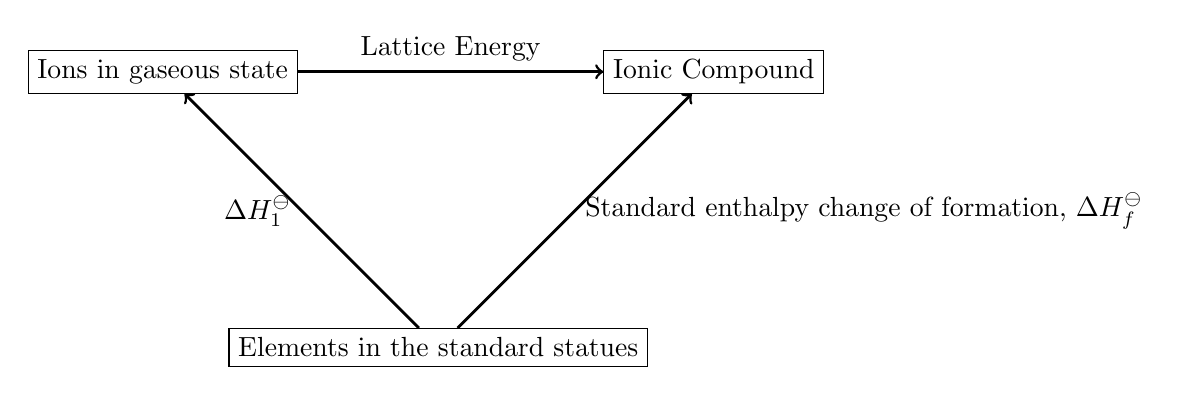
\begin{tikzpicture}[node distance=35mm]
		\node (ground) [rectangle, draw] {Elements in the standard statues};
		\node (ions) [rectangle, draw, above of=ground, left of=ground] {Ions in gaseous state};
		\node (comp) [rectangle, draw, above of=ground, right of=ground] {Ionic Compound};

		\draw[->, line width=1pt] (ground) -- node[left] {$\Delta H^\ominus_1$} (ions);	
		\draw[->, line width=1pt] (ground) to node[right] {Standard enthalpy change of formation, $\Delta H^\ominus_f$} (comp);
		\draw[->, line width=1pt] (ions) to node[auto] {Lattice Energy} (comp);

	\end{tikzpicture}
	\caption{Born-Haber Cycle}
	\label{bhc}
	\end{figure}

\section{Ion Polarisation}

	Sometimes the positive change on the cation in a ionic lattice may attract the electrons on the cation causing a distortion in the electron cloud. The anion is more likely to be polarised if:

	\begin{itemize}
		\item
			The cation is small or the anion is large.
		\item
			The cation has a large positive charge or the anion has a large negative charge.
	\end{itemize}

	\begin{figure}[h]
		\centering
		\caption{Ion Polarisation and distortion \cite{hrofchem}}
		\label{polar}
		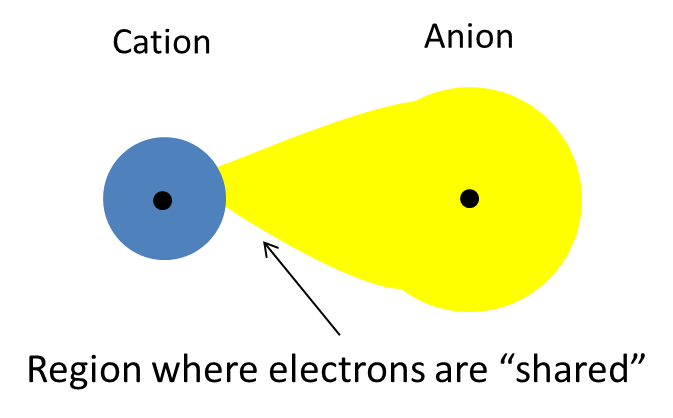
\includegraphics[width=0.5\linewidth]{assets/polar.png}
	\end{figure}

\section{Enthalpy changes in solution}

	\begin{quote}
		The enthalpy change of solution, $\Delta H^\ominus_{sol}$, is the energy absorbed or released when \SI{1}{\mole} of ionic solid dissolves in sufficient water to form a very dilute solution
	\end{quote}

	\[ \ce{MgCl(s) + aq -> Mg^{2+}(aq) + 2Cl-(aq) } \qquad \Delta H^\ominus_{sol} = \SI{-55}{\kilo\joule\per\mole} \]

	The value of $\Delta H^\ominus_{sol}$ is much less than $\Delta H^\ominus_{latt}$ because a lot of energy to overcome to lattice energycomes from the strong attraction between the ions and the molecules of water. This is called the enthalpy change of hydration.

	\begin{quote}
		The enthalpy change of hydration, $\Delta H^\ominus_{hyd}$, is the enthalpy change when \SI{1}{\mole} of a sepcified gaseous gaseous ion dissolves in sufficient water to form a very dilute solution
	\end{quote}

	\begin{figure}[h]
	\centering
	\caption{Hess diagram for $\Delta H^\ominus_{hyd}$}
	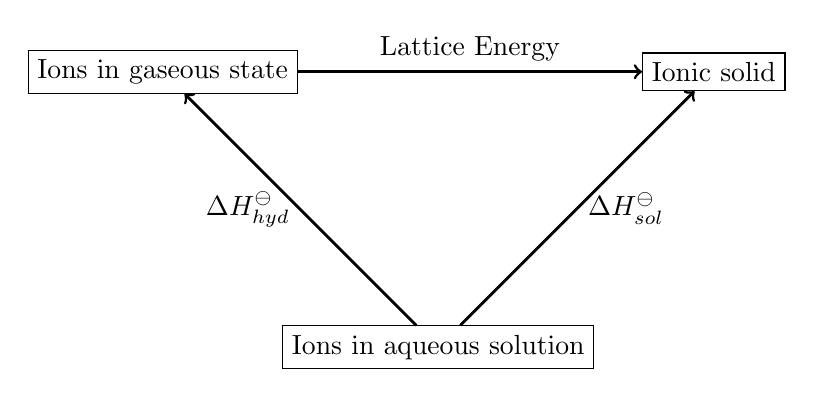
\begin{tikzpicture}[node distance=35mm]
                \node (ground) [rectangle, draw] {Ions in aqueous solution};
                \node (ions) [rectangle, draw, above of=ground, left of=ground] {Ions in gaseous state};
                \node (comp) [rectangle, draw, above of=ground, right of=ground] {Ionic solid};

			\draw[->, line width=1pt] (ground) -- node[left] {$\Delta H^\ominus_{hyd}$} (ions);
			\draw[->, line width=1pt] (ground) to node[right] {$\Delta H^\ominus_{sol}$} (comp);
                \draw[->, line width=1pt] (ions) to node[auto] {Lattice Energy} (comp);
	\end{tikzpicture}
	\end{figure}

	The decrease in solubility of Group 2 sulphates can be explained in terms of the relative values of the enthalpy change of hydration and the coresponding lattice energies.

\printbibliography{}
\end{document}
